%!TEX root = index.tex
\chapter[Requisitos]{Requisitos}
\label{chap:requisitos}

A partir dos objetivos deste Trabalho de Conclusão de Curso, é possível extrair os requisitos funcionais do sistema de recomendação. Esses requisitos ditam principalmente sobre a escalabilidade e o desempenho das recomendações do sistema.

Como as sugestões serão calculadas com antecedência, não há necessidade para uma elevada taxa de recomendações por período de tempo (\textit{throughput}). Deseja-se contudo que o sistema possa gerar todas as recomendações para um banco de dados de cem mil clientes em uma hora, isto é, que tenha \textit{throughput} mínimo de 28 recomendação por segundo. Os sistemas de recomendação tradicionais possuem \textit{throughput} de cerca de 500 recomendações por segundo, mas operam em servidores dedicados de maior potência computacional \cite{sarwar2001item}. 

A fim de poder estabelecer uma base comparativa entre o sistema proposto \textit{UI} e os sistemas de referência \textit{FW} e \textit{UP}, serão utilizados os mesmos indicadores de desempenho dos artigos-base: precisão, abrangência e medida $F_1$ \cite{symeonidis2007feature,debnath2008feature}. Precisão é a porcentagem de casos corretamente preditos em relação ao tamanho da lista de recomendações. Abrangência é a razão entre o número de itens corretamente preditos e daqueles que foram efetivamente avaliados pelo usuário. A medida $F_1$, por sua vez, é a média harmônica entre precisão e
abrangência.

Todas essas métricas são dependentes dos diversos parâmetros do problema, como do tamanho da lista de recomendações $N$, da quantidade de vizinhos mais próximos $k$, e principalmente do banco de dados de teste. Como os artigos de referência não os disponibilizaram integralmente, serão estimados os valores de precisão, abrangência e medida $F_1$ para o banco de dados da dupla. 

Espera-se que a precisão, abrangência e consequentemente a medida $F_1$ sejam maiores que 20\%. Esses valores foram escolhidos por serem superiores aos de algoritmos puramente baseados em conteúdo ou em filtragem colaborativa \cite{symeonidis2007feature,debnath2008feature}. Na prática, o resultado mais importante é a comparação entre os três métodos para um banco de dados de referência. 

Neste trabalho o \textit{benchmarking} é feito por meio da união de dois bancos amplamente utilizados na comunidade científica de Sistemas de Recomendação. O primeiro, denominado MovieLens 100k, é composto de 100 000 avaliações (valores inteiros de 1 a 5) de 943 usuários para 1682 filmes \cite{movielensdataset}. Além disso, cada usuário (idade, sexo, profissão, logradouro) avaliou pelo menos 20 filmes (categoria, ano de publicação). O segundo banco de dados é extraído do Internet Movie Database (IMDB), e possui 28 819 filmes. Esse banco está presente na biblioteca \texttt{ggplot2} da linguagem de programação R \cite{moviesggplot2dataset}. A união desses dois bancos é denominada 100k-IMDB, e a metodologia para essa união está descrita na Seção \ref{sec:modelamento_e_simula_o}.

Os requisitos funcionais são suportados por requisitos não-funcionais, e estes são determinados pelas restrições sobre o projeto ou execução, tais como desenvolvimento e confiabilidade.

O sistema de recomendação deverá poder ser utilizado por qualquer e-commerce que disponha de um banco de dados de clientes, produtos e histórico de compras, desde que o formato de entrada, a ser especificado no Capítulo \ref{chap:resultados}, seja seguido.

Além disso o sistema deverá ser desenvolvido em tecnologias abertas (\textit{open source}) que tenham um alto número de colaboradores, como o sistema de gestão de banco de dados MySQL ou a linguagem de programação estatística R, a fim de torná-lo reutilizável por alunos ou e-commerces interessados.

Por fim, o sistema de recomendação deverá ser escalável e flexível no sentido de poder operar igualmente bem tanto em pequenas quanto em grandes bases de dados.

Apesar serem importantes parâmetros de um sistema de recomendação, a taxa de recomendações por período de tempo e a escalabilidade estão intimamente relacionados ao orçamento do projeto. Pode-se obter virtualmente qualquer \textit{throughput} desejado, contanto que haja investimento equivalente em infra-estrutura computacional. O mesmo não é válido para os parâmetros de qualidade da recomendação, que dependem tão somente dos algoritmos de sugestão. Neste trabalho, assumimos que o sistema de operará em microcomputadores pessoais, e por isso o requisito funcional \textit{throughput} se faz necessário.

Com os requisitos do sistema de recomendação definidos, devemos estruturar o seu relacionamento com o administrador do sistema. Para isto determinamos as ações que o administrador pode realizar com este sistema. Cada uma destas ações é um caso de uso, e ao total foram criados nove casos de uso para este sistema.

O primeiro caso de uso é o caso \textit{Selecionar Método}, onde o administrador do sistema pode selecionar entre qual método de recomendação será utilizado para gerar as recomendações do sistema.

O segundo caso é o \textit{Selecionar Banco de Dados}, pelo qual é permitido ao administrador selecionar o banco de dados para o qual serão geradas as recomendações.

O terceiro caso \textit{Gerar Recomendações} é o caso onde o dá ínicio aos cálculos das recomendações com o método e o banco de dados préviamente escolhidos, o que caracteriza dependência indicada na figura.

O quarto caso de uso, \textit{Escolher Cliente}, permite ao administrador selecionar o cliente para o qual quer ter acesso às recomendações. Isto que nos leva ao quinto caso de uso, \textit{Ranquear Itens Para Cliente},o qual ordenas os itens do banco de dados de forma decrescente de acordo com o valor da recomendação para o cliente escolhido.

 O sexto caso, \textit{Avaliar Recomendações}, permite ao usuário avaliar a precisão de a acurácia do sistema. Este, em conjunto com o \textit{Fazer Validação Cruzada}, servirá para avaliar se o método utilizado para gerar as recomendações é indicado para ser implementado no sistema de vendas do e-commerce.

 O caso de uso \textit{Devolver Banco de Recomendações}, é o principal output do sistema, onde se devolve um banco de dados com todas as precisões de avaliações de cada um dos itens por cada um dos usuários.

 O último caso de uso, \textit{Devolver Pesos dos Atributos}, retornará o peso que cada atributo dos itens tem. Assim definindo quais atributos são mais importantes para cada usuário.

 Estes casos de uso foram representados no diagrama de casos de uso abaixo.

 \begin{figure}[htp]
    \begin{center}
    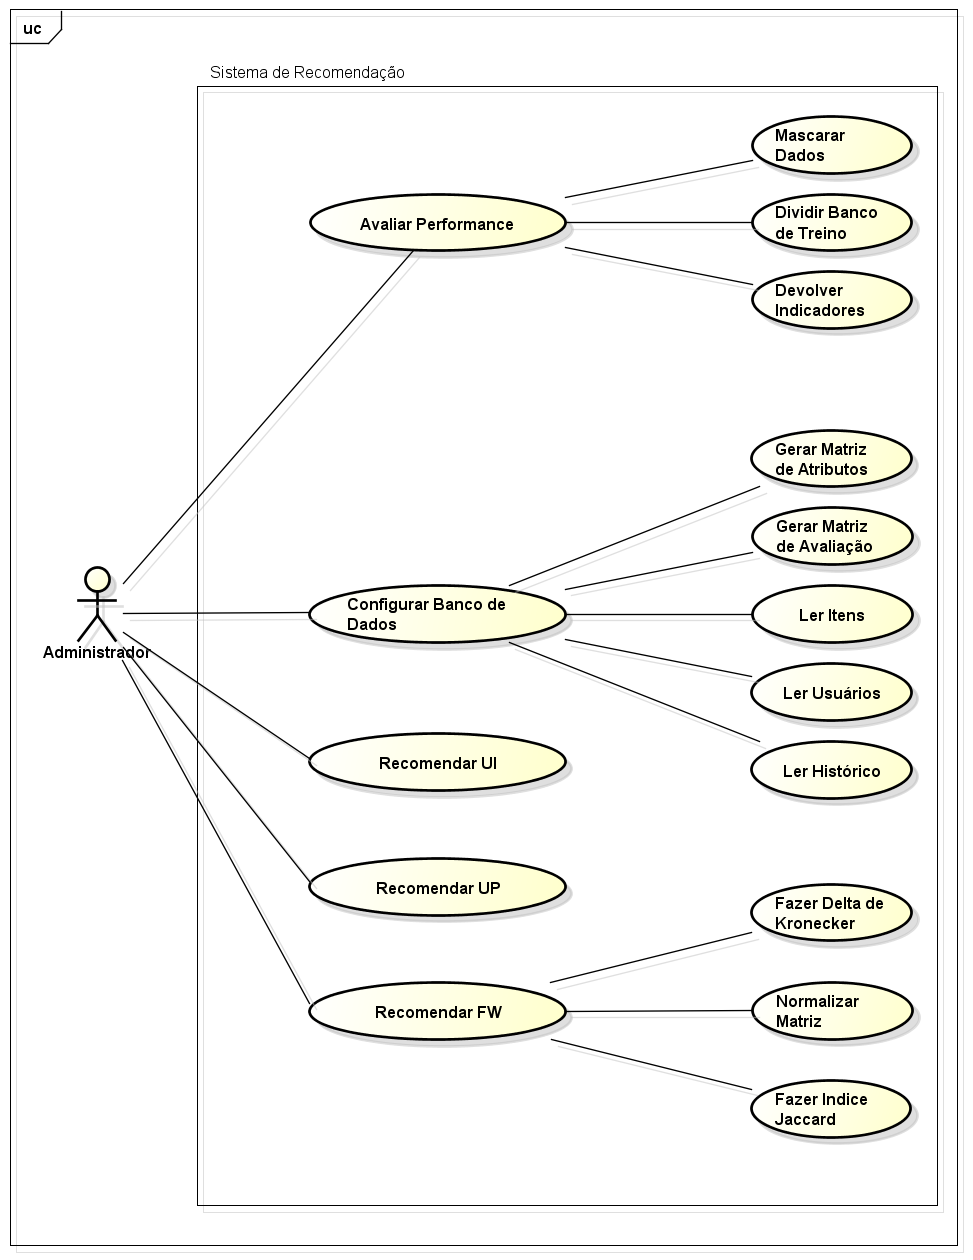
\includegraphics[width=1\textwidth]{img/CasosDeUso}
    \end{center}
    \label{fig:Diagrama de Casos de Uso}
    \caption{Diagrama de casos de uso representando os relacionamentos entre o administrador e o sistema.}
\end{figure}